\chapter{Applications}



\section{Oceanography}\label{sec:appl_ocean}

\subsection{Altimetry-derived velocity data}

Suppose we have the sea surface height (SSH) \(\eta = \eta\left(\lambda, \phi, t\right)\) at longitude \(\lambda\) and latitude \(\phi\) (both in radians), and at time \(t\).
The SSH \(\eta\) is then proportional to the streamfunction for the surface flow, if we treat the surface flow as two-dimensional, where the constant of proportionality varies with latitude \citep{Park_2004_DeterminationSurfaceGeostrophic, DoglioniEtAl_2021_SeaSurfaceHeight}.
The geostrophic zonal (east-west) and meridional (north-south) velocities \(u\) and \(v\) are then given by
\begin{subequations}\label{eqn:}
	\begin{align}
		u\left(\lambda, \phi, t\right) & = -\frac{g}{f\left(\phi\right)}\dpd{\eta}{\phi} \label{eqn:altimetry_u}    \\
		v\left(\lambda, \phi, t\right) & = \frac{g}{f\left(\phi\right)}\dpd{\eta}{\lambda} \label{eqn:altimetry_v},
	\end{align}
\end{subequations}
\label{eqn:altimetry_uv}
where
\[
	f\left(\phi\right) = 2\Omega_{\mathrm{r}}\sin{\phi}
\]
is the Coriolis parameter, \(g \approx 9.81\mathrm{\,m\,s}^{-1}\) is the standard acceleration due to gravity, and \(\Omega_\mathrm{r} \approx 7.2921 \times 10^{-5}\mathrm{\,radians\,s}^{-1}\) is the rotation rate of the Earth.


\Cref{fig:na_snapshots} shows contours of the sea surface height at several different times within the interval and domain of interest.

\begin{figure}
	\begin{center}
		% \includegraphics[width=\textwidth]{}
		\caption{}
		\label{fig:na_snapshots}
	\end{center}
\end{figure}





To account for measurement error, we consider the evolution of the following stochastic model
\begin{equation}
	\dif \begin{bmatrix}
			x^{(\mathrm{lon})}_t \\ x^{(\mathrm{lat})}_t
		\end{bmatrix} = \begin{multlined}[t]
			\begin{bmatrix} u\left(x^{(\mathrm{lon})}_t, x^{(\mathrm{lat})}_t, t\right) \\ v\left(x^{(\mathrm{lon})}_t, x^{(\mathrm{lat})}_t, t\right) \end{bmatrix}\dif t \\
				+ L_r\begin{bmatrix}
			\sqrt{u_{\mathrm{err}}\left(x^{(\mathrm{lon})}_t, x^{(\mathrm{lat})}_t, t\right)} & 0                                                                                 \\
			0                                                                                 & \sqrt{v_{\mathrm{err}}\left(x^{(\mathrm{lon})}_t, x^{(\mathrm{lat})}_t, t\right)}
		\end{bmatrix} \dif W_t,
\end{multlined}
	\label{eqn:natl_sde}
\end{equation}
where \(t\) is the time in days from DATE, \(u\) and \(v\) are the interpolated zonal and meridional velocities (in \(\mathrm{\,degrees\,day}^{-1}\)), \(u_{\mathrm{err}}\) and \(v_{\mathrm{err}}\) are the respective interpolated error estimates (in \(\mathrm{\,degrees\,day}^{-1}\)), and \(L_r = 0.25 \mathrm{\,degrees}\) is the spatial resolution of the data.



The derivatives of the deterministic velocity field in \eqref{eqn:natl_sde} are approximated via the centred finite-differences
\begin{align*}
	\dpd{u\left({x^{(\text{lon})}}, {x^{(\text{lat})}}, t\right)}{{x^{(\text{lon})}}} & \approx \frac{u\left(x^{(\text{lon})} + L_r, x^{(\text{lat})}, t\right) - u\left(x^{(\text{lon})} - L_r, x^{(\text{lat})}, t\right)}{2 L_r},
\end{align*}
and similar for the remaining derivatives.


\subsection{The Gulf Stream}\label{sec:gulf_stream}


\subsubsection{A motivating example}



\begin{figure}
	\begin{center}
		\begin{subfigure}{0.8\textwidth}
			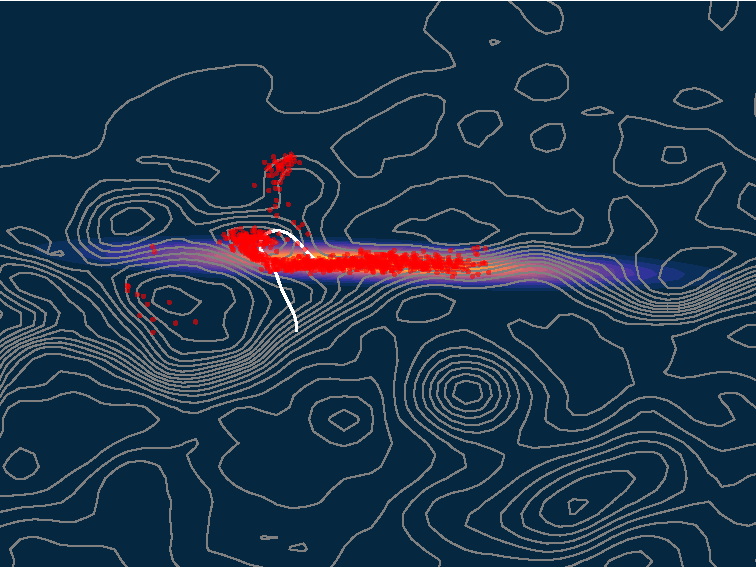
\includegraphics[width=\textwidth]{figures/gulf_stream_motivation/single_gaussian.pdf}
			\caption{Each sample is represented by a single red marker.}
			\label{fig:}
		\end{subfigure}
		\begin{subfigure}{0.8\textwidth}
			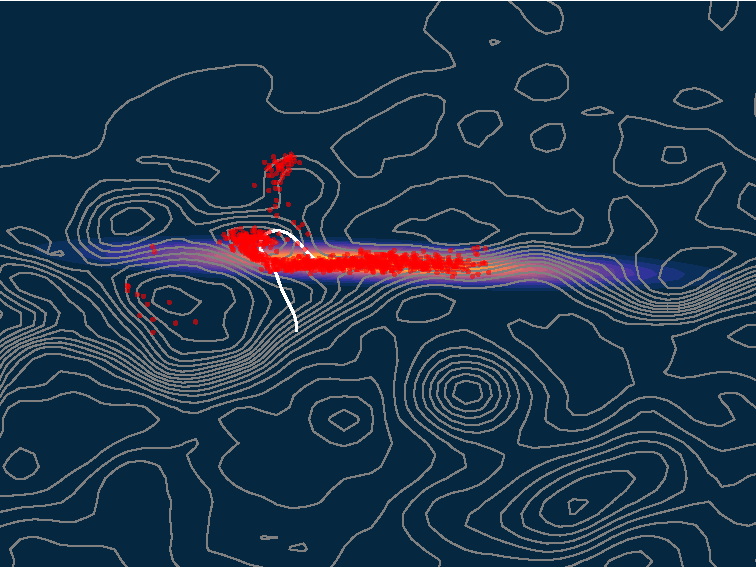
\includegraphics[width=\textwidth]{figures/gulf_stream_motivation/single_gaussian.pdf}
			\caption{The samples are binned into a histogram, with contours of the Gaussian PDF overlaid.}
			\label{fig:}
		\end{subfigure}
		\caption{Comparison of stochastic}
	\end{center}
\end{figure}




\subsection{The Southern Ocean}

\section{Atmospheric regimes}


\subsection{Multiplicative noise regime}


We consider the example consider by \citet{SuraEtAl_2005_MultiplicativeNoiseNonGaussianity}, in which a stochastic differential equation linear dynamics but multiplicative noise is used to model the time-evolution of the observed streamfunction of the

The linearity of the deterministic dynamics means that the flow map \(F_s^t\) is available analytically, and so we can compute the limiting covariance exactly by using the alternative expression \eqref{eqn:sigma_calc}.
However, the observed data itself displays non-Gaussianity, so the introduction of multiplicative noise is necessary to capture this.




\section{Epidemiology}
